\documentclass{beamer}

\usepackage[frenchb]{babel}
\usepackage[utf8x]{luainputenc}
\usepackage{graphicx}
\usepackage{tikz}
\usepackage{subcaption}
\usetikzlibrary{graphdrawing,graphs}
\usegdlibrary{layered}
\usegdlibrary{force}

% There are many different themes available for Beamer. A comprehensive
% list with examples is given here:
% http://deic.uab.es/~iblanes/beamer_gallery/index_by_theme.html
% You can uncomment the themes below if you would like to use a different
% one:
%\usetheme{AnnArbor}
%\usetheme{Antibes}
%\usetheme{Bergen}
%\usetheme{Berkeley}
%\usetheme{Berlin}
%\usetheme{Boadilla}
%\usetheme{boxes}
%\usetheme{CambridgeUS}
%\usetheme{Copenhagen}
%\usetheme{Darmstadt}
\usetheme{default}
%\usetheme{Frankfurt}
%\usetheme{Goettingen}
%\usetheme{Hannover}
%\usetheme{Ilmenau}
%\usetheme{JuanLesPins}
%\usetheme{Luebeck}
%\usetheme{Madrid}
%\usetheme{Malmoe}
%\usetheme{Marburg}
%\usetheme{Montpellier}
%\usetheme{PaloAlto}
%\usetheme{Pittsburgh}
%\usetheme{Rochester}
%\usetheme{Singapore}
%\usetheme{Szeged}
%\usetheme{Warsaw}

\title{Jeu multi-joueurs sur les graphes d'argumentation}
\author{Alexis Martin\\encadré par Elise Bonzon et Nicolas Maudet}
\titlegraphic{
  \includegraphics[width=2cm]{images_presentation/logos/p7.png}\hspace*{2.25cm}~%
  \includegraphics[width=1.5cm]{images_presentation/logos/lip6.png}
  \hspace*{2.25cm}~%
  \includegraphics[width=2cm]{images_presentation/logos/upmc.png}
}
\date{07 septembre 2016}
% Let's get started
\begin{document}

  \begin{frame}
    \titlepage
  \end{frame}

    \begin{frame}{Introduction}
      \noindent
     \begin{minipage}[c]{.46\linewidth}
       Les graphes d'argumentation.
        \begin{itemize}
          \item Formalisation mathématiques d'un débat.
          \item L'analyse automatique d'un débat, d'arguments.
        \end{itemize}
        \vspace{1em}

        \textbf{Plan}
        \vspace{0.3em}
        \tableofcontents
     \end{minipage} \hfill
     \begin{minipage}[c]{.5\linewidth}
       \begin{figure}
        \includegraphics[scale=0.3]{images_presentation/debateGraph.png}
          \caption{www.debategraph.org}
        \end{figure}
     \end{minipage}
    \end{frame}

  \section{Les graphes d'argumentation}
  \begin{frame}{Les graphes d'argumentation}
      \noindent
     \begin{minipage}[c]{.6\linewidth}
       Un graphe d'argumentation valué est un tuple $F = \langle \mathcal{A}, \mathcal{R}, V \rangle$
       \begin{itemize}
         \item $\mathcal{A}$ : L'ensemble des arguments.
         \item une question $q \in \mathcal{A}$.
         \item $\mathcal{R} \subseteq \mathcal{A} \times \mathcal{A}$ : $(a,b) \in \mathcal{R}$ si $a$ "attaque" $b$.
         \item $V: \mathcal{A} \rightarrow \mathbb{N} \times \mathbb{N} : V(a) = (v^+, v^-)$ signifie que $a$ à $v^+$ "like" et $v^-$ "dislike".
       \end{itemize}
     \end{minipage} \hfill
     \begin{minipage}[c]{.35\linewidth}
       \begin{overprint}
         \onslide<1>
         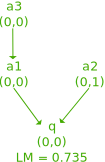
\includegraphics[scale=0.7]{images_presentation/graphe1.png}
         \onslide<2>
         \includegraphics[scale=0.7]{images_presentation/graphe1_r.png}
         \onslide<3>
         \includegraphics[scale=0.7]{images_presentation/graphe1_b.png}
       \end{overprint}
     \end{minipage}
  \end{frame}

  \section{SAF}

  \begin{frame}{Social Argumentation Framework (SAF)\footnote{J. Leite, J. Martins - Social Abstract Argumentation - \emph{Proc. of IJCAI’11}}}
    Modèle permettant de calculer une préférence sur les arguments.

    \begin{itemize}
      \onslide<1->
      \item La fonction d'agrégation des votes.
      $\tau_\varepsilon : \mathcal{A} \rightarrow [0, 1]$ par :

      $$
      \tau_\varepsilon(a) = \left\{
          \begin{array}{lll}
            0 & \mbox{si } & v^+ = v^- = 0\\
            \frac{v^+}{v^+ + v^- + \varepsilon} & \mbox{sinon} & \\
          \end{array}\right.$$

        Avec $\varepsilon \geq 0$.

      \onslide<2->
      \item La sémantique simple product semantics

      C'est un tuple $\mathcal{S}_\varepsilon = \langle [0, 1], \tau_\varepsilon, \curlywedge, \curlyvee, \neg  \rangle$ tel que :
      \begin{enumerate}
        \item $x_1 \curlywedge x_2 = x_1 \cdot x_2$
        \item $x_1 \curlyvee x_2 = x_1 + x_2 - x_1 \cdot x_2$
        \item $\neg x_1 = 1 - x_1$
        \item $\varepsilon \geq 0$
      \end{enumerate}

      \item Social Model

      $LM(a) = \tau(a) \curlywedge \neg$ {\Large $\curlyvee$} $\{LM(a_i)\ |\ a_i \in Att(a)\}$
    \end{itemize}
  \end{frame}

  \begin{frame}{Social Argumentation Framework}
    \begin{overprint}
      \onslide<1-2>
      $$
      \tau_\varepsilon(a) = \left\{
          \begin{array}{lll}
            0 & \mbox{si } & v^+ = v^- = 0\\
            \frac{v^+}{v^+ + v^- + \varepsilon} & \mbox{sinon} & \\
          \end{array}\right.$$

      \onslide<3->
      $LM(a) = \tau(a) \curlywedge \neg$ {\Large $\curlyvee$} $\{LM(a_i)\ |\ a_i \in Att(a)\}$
    \end{overprint}


    \begin{minipage}[c]{.6\linewidth}
      \begin{overprint}
        \onslide<1>
        \begin{tabular}{|c|c|c|}
          \hline
          & $\tau$ & $LM$\\
          \hline
          a1 & $\frac{1}{4+1+0.1}$ & \\
          \hline
          a2 & & \\
          \hline
          a3 & & \\
          \hline
          a4 & & \\
          \hline
          a5 & & \\
          \hline
          q & & \\
          \hline
        \end{tabular}
        \onslide<2>
        \begin{tabular}{|c|c|c|}
          \hline
          & $\tau$ & $LM$\\
          \hline
          a1 & $\frac{1}{5.1}$ & \\
          \hline
          a2 & $\frac{2}{5.1}$ & \\
          \hline
          a3 & $\frac{1}{2.1}$ & \\
          \hline
          a4 & $\frac{1}{1.1}$ & \\
          \hline
          a5 & $0$ & \\
          \hline
          q & $0$ & \\
          \hline
        \end{tabular}
        \onslide<3>
        \begin{tabular}{|c|c|c|}
          \hline
          & $\tau$ & $LM$\\
          \hline
          a1 & $\frac{1}{5.1}$ & \\
          \hline
          a2 & $\frac{2}{5.1}$ & $\frac{2}{5.1}$ \\
          \hline
          a3 & $\frac{1}{2.1}$ & \\
          \hline
          a4 & $\frac{1}{1.1}$ & $\frac{1}{1.1}$\\
          \hline
          a5 & $0$ & 0\\
          \hline
          q & $0$ & \\
          \hline
        \end{tabular}
        \onslide<4>
        \begin{tabular}{|c|c|c|}
          \hline
          & $\tau$ & $LM$\\
          \hline
          a1 & $\frac{1}{5.1}$ & $0.005675$\\
          \hline
          a2 & $\frac{2}{5.1}$ & $\frac{2}{5.1}$ \\
          \hline
          a3 & $\frac{1}{2.1}$ & $0.47619$\\
          \hline
          a4 & $\frac{1}{1.1}$ & $\frac{1}{1.1}$\\
          \hline
          a5 & $0$ & 0\\
          \hline
          q & $0$ & 0\\
          \hline
        \end{tabular}
      \end{overprint}

    \end{minipage}\hfill
    \begin{minipage}[c]{.35\linewidth}
    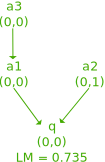
\includegraphics[scale=0.7]{images_presentation/graphe1.png}
  \end{minipage}
    \end{frame}

    \section{Notre jeu}
  \begin{frame}{Le modèle}{Principe général}
    \begin{itemize}
      \item Un débat est terminé et on a un graphe d'argumentation représentant ce débat.
      \item On a $n$ agents qui ont connaissance du graphe.
      \item Chaque agent à un avis personnel sur chacun des arguments ainsi que sur la question.
      \item Ils vont voter chacun leurs tour sur un argument jusqu'à arriver à un consensus.
      \item Cela nous donne un résultat sur la question du débat.
    \end{itemize}
  \end{frame}

  \begin{frame}{Le modèle}{Valeur intrinsèque des joueurs}
    \begin{itemize}
      \item Chacun des agents vote de façon personnelle sur l'ensemble des arguments.
      \item On calcule la valeur de la question grâce au SAF.

      On appelle cette valeur, la valeur du joueur.
      \item L'objectif de chaque agent est que la valeur de la question soit la plus proche possible de leur valeur.
    \end{itemize}

    \begin{figure}
      \centering
      \begin{subfigure}{.3\linewidth}
        \centering
          \includegraphics[scale=0.7]{images_presentation/graphe2_j1_lm.png}

      \end{subfigure}
      \hskip1em
      \begin{subfigure}{.3\linewidth}
        \centering
          \includegraphics[scale=0.7]{images_presentation/graphe2_j2_lm.pdf}
      \end{subfigure}
      \hskip1em
      \begin{subfigure}{.3\linewidth}
        \centering
          \includegraphics[scale=0.7]{images_presentation/graphe2_j3_lm.png}
      \end{subfigure}
    \end{figure}

  \end{frame}

  \begin{frame}{Le modèle}{Le jeu}
    \noindent
    \begin{minipage}{.14\linewidth}
      \begin{figure}
            \includegraphics[scale=0.45]{images_presentation/graphe2_j1_lm.png}
        \end{figure}
        \vskip-1.5em
        \begin{figure}
            \includegraphics[scale=0.45]{images_presentation/graphe2_j2_lm.pdf}
        \end{figure}
        \vskip-1.5em
      \begin{figure}
            \includegraphics[scale=0.45]{images_presentation/graphe2_j3_lm.png}
      \end{figure}
    \end{minipage}\hfill
    \begin{minipage}[c]{.16\linewidth}
      \begin{overprint}
        \onslide<1>
        \includegraphics[scale=0.7]{images_presentation/graphe2_0.png}
        \onslide<2>
        \includegraphics[scale=0.7]{images_presentation/graphe2_1.pdf}
        \onslide<3>
        \includegraphics[scale=0.7]{images_presentation/graphe2_2.pdf}
        \onslide<4>
        \includegraphics[scale=0.7]{images_presentation/graphe2_3.pdf}
        \onslide<5>
        \includegraphics[scale=0.7]{images_presentation/graphe2_4.pdf}
      \end{overprint}

    \end{minipage}\hfill
    \begin{minipage}[c]{.67\linewidth}

    \begin{itemize}

      \item On commence le jeu avec le graphe sans vote et on calcule la valeur du jeu.

      \item La valeur du jeu est la valeur de la question.
      \item Aucun vote sur la question.
      \item A son tour un joueur choisi entre :
        \begin{itemize}
          \item Voter sur un "nouvel" argument.
          \item Changer, ou annuler un de ses votes précédents.
          \item Ne rien faire.
        \end{itemize}
          \item La valeur du jeu est recalculée après chaque action d'un joueur.
    \end{itemize}
  \end{minipage}
  \end{frame}

  \begin{frame}{Le modèle}{La dynamique du jeu}

    La dynamique du jeu est constitué de deux aspects :\\

    \begin{enumerate}
      \item Choix du joueur suivant :
        \begin{itemize}
          \item Random
          \item Round Robin\\
        \end{itemize}

      \item La stratégie des joueurs.
        \begin{itemize}
          \item Best response
          \item Better response
        \end{itemize}
    \end{enumerate}
  \end{frame}

  \section{Recherche et contribution}
  \begin{frame}{Question de recherche et contribution}
    \begin{itemize}
      \item Problèmes liés au modèle.
      \item Convergence du jeu sur différentes classes de graphe.
      \item Caractériser la qualité des solutions.
      \item Implémentation d'une plate-forme de tests.
  \end{itemize}

  On dit qu'un jeu possède la \textbf{convergence garantie} si toutes les parties possibles sur ce jeu sont finies. C'est à dire qu'il n'y a pas de cycle.

  On dit qu'il possède la \textbf{convergence à la limite} si pour toutes les parties il existe un équilibre atteignable.
  \end{frame}

  \begin{frame}{Problèmes liés au modèle}
    \begin{itemize}
      \item La question à toujours une valeur égale à 0.
      \item Un argument qui n'a que des votes négatifs aura une valeur égale à 0.
    \end{itemize}


    $$
        \left\{\begin{array}{llll}
          \tau(q) & = & 1 & \\
          \tau(a) & = & \frac{1}{2} \cdot \left(1 + sgn(v^+ - v^-) \cdot \left(1 - e^{\frac{-|v^+ - v^-|}{\varepsilon}}\right)\right)
        \end{array}\right.
      $$

      \includegraphics[scale=0.5]{images_presentation/Laplace.png}
  \end{frame}

  \begin{frame}{Résultats}{Les graphes cycliques et acycliques}
    La convergence n'est pas assurée.
    \begin{figure}
    	  	\centering

            \begin{subfigure}{.32\linewidth}
            	\centering
                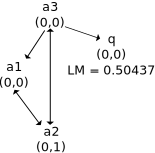
\includegraphics[scale=0.6]{images_presentation/graphe3_j1.pdf}
                \caption{Graphe du joueur 1}
			\end{subfigure}
            \hskip2em
            \begin{subfigure}{.5\linewidth}
            	\centering
                \includegraphics[scale=0.6]{images_presentation/graphe3_j2.pdf}
                \caption{Graphe du joueur 2}
			\end{subfigure}
	    	\begin{subfigure}{.25\linewidth}
            	\centering
            		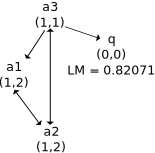
\includegraphics[scale=0.6]{images_presentation/graphe3.pdf}
                \caption{Graphe du jeu}
			\end{subfigure}
          	\hskip1.32em
          	\begin{subfigure}{.5\linewidth}
              \begin{footnotesize}
    		\begin{tabular}{|c|c|c|c|}
          \hline
          & joueur 1 & joueur 2 & general \\
          \hline
          tour 1 & \_ & \_ & 0.59680 \\
          \hline
          tour 4 & \_ & a1 like & 0.60259 \\
          \hline
          \textcolor{red}{tour 5} & \textcolor{red}{a1 dislike} & \textcolor{red}{\_} & \textcolor{red}{0.59680} \\
          \hline
          tour 6 & \_ & a1 dislike & 0.60493 \\
          \hline
          tour 7 & a1 like & \_ & 0.59680 \\
          \hline
          tour 8 & \_ & a1 like & 0.60493 \\
          \hline
          \textcolor{red}{tour 9} & \textcolor{red}{a1 dislike} & \textcolor{red}{\_} & \textcolor{red}{0.59680} \\
          \hline
                \end{tabular}
              \end{footnotesize}
			\end{subfigure}
            \label{fig:graph_cycle}
		\end{figure}

  \end{frame}

  \begin{frame}{Résultats}{Les graphes non ambigüs}

    Un argument \textbf{ambigü} est un argument qui attaque la question par un chemin et la défend par un autre.
    \begin{overprint}

      \onslide<1>
      \begin{figure}
        \centering
      \includegraphics[scale=0.6]{images_presentation/graphe3_r.pdf}
      \end{figure}
      \onslide<2->
      \begin{figure}
        \centering
      \includegraphics[scale=0.6]{images_presentation/graphe3_b.pdf}
    \end{figure}
    \end{overprint}

    \onslide<3->
    Un \textbf{graphe non ambigü} est un graphe qui ne possède pas d'argument ambigü.

\vspace{2em}
    \textbf{Remarque :} Un graphe non ambigü est un graphe biparti.
  \end{frame}

  \begin{frame}{Résultats}{Convergence sur les arbres}
    Les expériences (plus de 30 millions de tests) semblent valider :
    \begin{tabular}{|c|c|c|}
      \hline
      & \textbf{Best response} & \textbf{Better response} \\
      \hline
      \textbf{Round Robin} & convergence garantie & convergence garantie \\
      \hline
      \textbf{Random} & convergence garantie & convergence à la limite \\
      \hline
    \end{tabular}
    \vspace{1em}

    \textbf{Conjecture :} Si on munit un jeu, sur un graphe non ambigü, d'une dynamique
    \begin{itemize}
      \item \emph{Round Robin}, \emph{Best response}
      \item \emph{Round Robin}, \emph{Better response}
      \item \emph{Random}, \emph{Best response}
    \end{itemize}
    Alors le jeu possède la \textbf{convergence garantie}.
    \vspace{1em}

    \textbf{Conjecture :} Si on munit un jeu, sur un graphe non ambigü, de la dynamique \emph{Random}, \emph{Better response}
    Alors le jeu possède la \textbf{convergence à la limite}.
  \end{frame}

  \begin{frame}{Résultats}{Les graphes non ambigüs}
    \begin{itemize}
      \item<1-> A deux joueurs, avec la dynamique Round robin et la stratégie Best response, si la valeur initiale est entre min et max alors on converge vers cette valeur.
      \item<2-> Il existe des états d'équilibre qui ne sont pas entre le min et le max.
      \item<3-> A 1 joueur, la valeur finale du jeu n'est pas toujours égale à la valeur du joueur.
    \end{itemize}

    \begin{overprint}
      \onslide<3>
        \begin{figure}
          \centering
          \begin{subfigure}{.45\linewidth}
            \begin{tikzpicture}[>=stealth]
              \graph [ layered layout, nodes = {scale=0.60, align=center} ] {
              "a1\\ (0,1)" -> "q\\ (0,0)\\lm = 0.48491";
              "a2\\ (0,0)" -> "q\\ (0,0)\\lm = 0.48491";
              "a3\\ (0,1)" -> "q\\ (0,0)\\lm = 0.48491";
              "a4\\ (1,0)" -> "a2\\ (0,0)";
              "a5\\ (1,0)" -> "a3\\ (0,1)";
              "a6\\ (0,0)" -> "q\\ (0,0)\\lm = 0.48491";
              };
            \end{tikzpicture}
            \caption {graphe du Joueur \textcolor{red}{$LM = 0.48491$}}
  			\end{subfigure}
        \begin{subfigure}{.45\linewidth}
          \begin{tikzpicture}[>=stealth]
            \graph [ layered layout, nodes = {scale=0.60, align=center} ] {
            "a1\\ (0,1)" -> "q\\ (0,0)\\lm = 0.54022";
            "a2\\ (0,0)" -> "q\\ (0,0)\\lm = 0.54022";
            "a3\\ (0,0)" -> "q\\ (0,0)\\lm = 0.54022";
            "a4\\ (0,0)" -> "a2\\ (0,0)";
            "a5\\ (0,0)" -> "a3\\ (0,0)";
            "a6\\ (0,1)" -> "q\\ (0,0)\\lm = 0.54022";
            };
          \end{tikzpicture}
          \caption {graphe du Jeu \textcolor{red}{$LM = 0.54022$}}
        \end{subfigure}
        \end{figure}


      \onslide<2>
      \begin{center}
        \includegraphics[scale=0.50]{/home/talkie/Documents/Stage/DebateGames/docs/examples/not_in_range_tau_1.png}
      \end{center}


      \onslide<1>
      L'intuition est qu'a chaque coup, le joueur qui joue peut assurer une valeur du jeu située entre sa valeur et la valeur initiale.
      \includegraphics[scale = 0.7]{images_presentation/graphe4.pdf}

    \end{overprint}
  \end{frame}

  \begin{frame}{Campagne de tests}
    Faire des tests pour analyser la qualité de la solution:
    \begin{itemize}
      \item Existe-t-il un rapport entre la question et la moyenne des valeurs des joueurs? L'agrégation des votes des joueurs?
      \item Quel est le pourcentage de jeu qui ont une valeur finale entre min et max.

    \end{itemize}
  \end{frame}

  \begin{frame}{conclusion}
    \begin{itemize}
      \item Ce modèle multi-agents permet d'avoir une nouvelle approche dans l'évaluation des débats.
      \item Des tests qui sont concluant sur les graphes sans argument ambigü.
      \item Afin de garantir la convergence sur tous les graphes on pourrait remplacer la valeur des joueurs par un intervalle.
    \end{itemize}
  \end{frame}

\end{document}
